%%%%%%%%%%%%%%%%%%%%%%%%%%%%%%%%%%%%%%%%%

%%%%%%%%%%%%%%%%%%%%%%%%%%%%%%%%%%%%%%%%%

%----------------------------------------------------------------------------------------
%	PACKAGES AND OTHER DOCUMENT CONFIGURATIONS
%----------------------------------------------------------------------------------------

\documentclass[final]{beamer}
\usepackage{bigints}

\usepackage{graphicx} % Required for including images
\graphicspath{{figures/}} % Location of the graphics files
\usepackage{booktabs} % Top and bottom rules for table
\usepackage[font=small,labelfont=bf]{caption} % Required for specifying captions to tables and figures
\usepackage{amsfonts, amsmath, amsthm, amssymb} % For math fonts,  symbols and environments
\usepackage{wrapfig} % Allows wrapping text around tables and figures
\theoremstyle{plain}
\newtheorem{thm}{Theorem}[section]

\newtheorem{prop}[thm]{Proposition}
\newtheorem*{cor}{Corollary}

\theoremstyle{definition}

\newtheorem{conj}{Conjecture}[section]
\newtheorem{exmp}{Example}[section]

\newtheorem{defn}{Definition}[subsection]
\theoremstyle{remark}
\newtheorem*{rem}{Remark}
\usepackage{mathpazo}
\usepackage{mdframed} %Allows text boxes and text background
\usepackage{xcolor}%extends the range of specified colours
\usepackage{float}
\usepackage[scale=1.24]{beamerposter} % Use the beamerposter package for laying out the poster

\usetheme{confposter} % Use the confposter theme supplied with this template
\usepackage{exscale} %allows integrals to be rescaled

\setbeamercolor{block title}{fg=white,bg=Violet} % Colors of the block titles
\setbeamercolor{block body}{fg=black,bg=Periwinkle} % Colors of the body of blocks

\setbeamercolor{block alerted title}{fg=white,bg=dblue!90} % Colors of the highlighted block titles
\newcommand{\blockcaption}{Periwinkle}
\newcommand{\blockitem}{Periwinkle}
\newcommand{\alertblockcaption}{black}
\newcommand{\alertblockitem}{black}
\setbeamercolor{block alerted body}{fg=black,bg=dblue!25} % Colors of the body of highlighted blocks
% Many more colors are available for use in beamerthemeconfposter.sty
\setbeamertemplate{caption}[numbered]{}
%-----------------------------------------------------------
% Define the column widths and overall poster size
% To set effective sepwid, onecolwid and twocolwid values, first choose how many columns you want and how much separation you want between columns
% In this template, the separation width chosen is 0.024 of the paper width and a 4-column layout
% onecolwid should therefore be (1-(# of columns+1)*sepwid)/# of columns e.g. (1-(4+1)*0.024)/4 = 0.22
% Set twocolwid to be (2*onecolwid)+sepwid = 0.464
% Set threecolwid to be (3*onecolwid)+2*sepwid = 0.708

\newlength{\sepwid}
\newlength{\firstcolwid}
\newlength{\twocolwid}
\newlength{\threecolwid}
\newlength{\logoheight}
\setlength{\paperwidth}{33.1in} % A0 width: 46.8in
\setlength{\paperheight}{46.8in} % A0 height: 33.1in
\setlength{\sepwid}{0.02\paperwidth} % Separation width (white space) between columns
\setlength{\firstcolwid}{0.3\paperwidth} %width of first column
\setlength{\twocolwid}{0.3\paperwidth} % Width of second column
%\setlength{\twocolwid}{0.4\paperwidth} % Width of two columns
\setlength{\threecolwid}{0.3\paperwidth} % Width of thired columns
\setlength{\logoheight}{0.03\paperheight}
%\setlength{\topmargin}{-0.5in} % Reduce the top margin size

 \newcommand{\PDE}{Partial differential equation }
 \newcommand{\pde}{partial differential equation }
 \newcommand{\vertspace}{\vspace{0.75cm}}
 \newcommand{\logospace}{\hspace{0.01\linewidth}}
 
%-----------------------------------------------------------
\usepackage{environ}
\usepackage{varwidth}
\usepackage{lipsum}
\usepackage{graphicx}  % Required for including images
\usepackage{amssymb}
\usepackage{amsbsy}
\usepackage{mathrsfs}
\usepackage{booktabs} % Top and bottom rules for tables
\usepackage{multicol}
\usepackage[export]{adjustbox}
\usepackage{eso-pic}
\usepackage{mdframed}

%----------------------------------------------------------------------------------------
%	TITLE SECTION 
%----------------------------------------------------------------------------------------
\columnsep=20pt % This is the amount of white space between the columns in the poster
\columnseprule=5pt

%%%%%%%%%%%%%%%%%%%%%%%EDITEDIT
% Fill in the following fields for the title section. 
% To format the display of the title section you will need to edit the style file beamerconfposter.sty.
\title{The Method of Geometric Optics and the Application to High-Frequency Wave Propagation.} % Poster title 
\author{Hayley Wragg \href{mailto:h.wragg@bath.ac.uk}{H.Wragg@bath.ac.uk} } % Author(s)
\def \photo{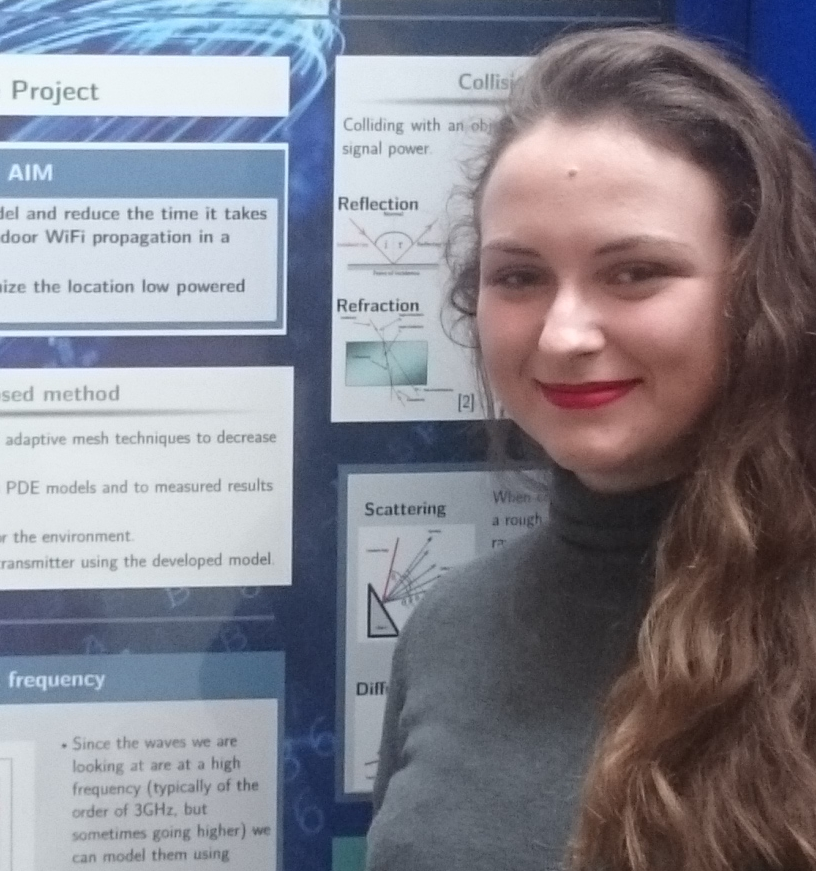
\includegraphics[width=\linewidth]{HWragg}}
\def \supervisor{Prof. C. J. Budd, Dr. R. Watson}
\def \cosupervisor{Dr. K. Briggs, Dr. M. Fitch}
\institute{University of Bath} % Institution
 \def \event{ \ }
 \def \logo{  
 
\includegraphics[height=\logoheight]{50th-anniversary-logo.png} \logospace 
 
\includegraphics[height=\logoheight]{BT.jpg} \logospace
 
\includegraphics[height=\logoheight]{smithlogo-full.png} \logospace 
 
\includegraphics[height=\logoheight]{samba.png} \logospace 
 
\includegraphics[height=\logoheight]{imilogo.jpg} }


%----------------------------------------------------------------------------------------

\begin{document}
%%%%%%%%%%%%%%%%%%%%%%%EDITEDIT 
% To change the background image\usebackgroundtemplate{\includegraphics[width=\paperwidth, height=\paperheight]{INSERT IMAGE NAME}
%\usebackgroundtemplate{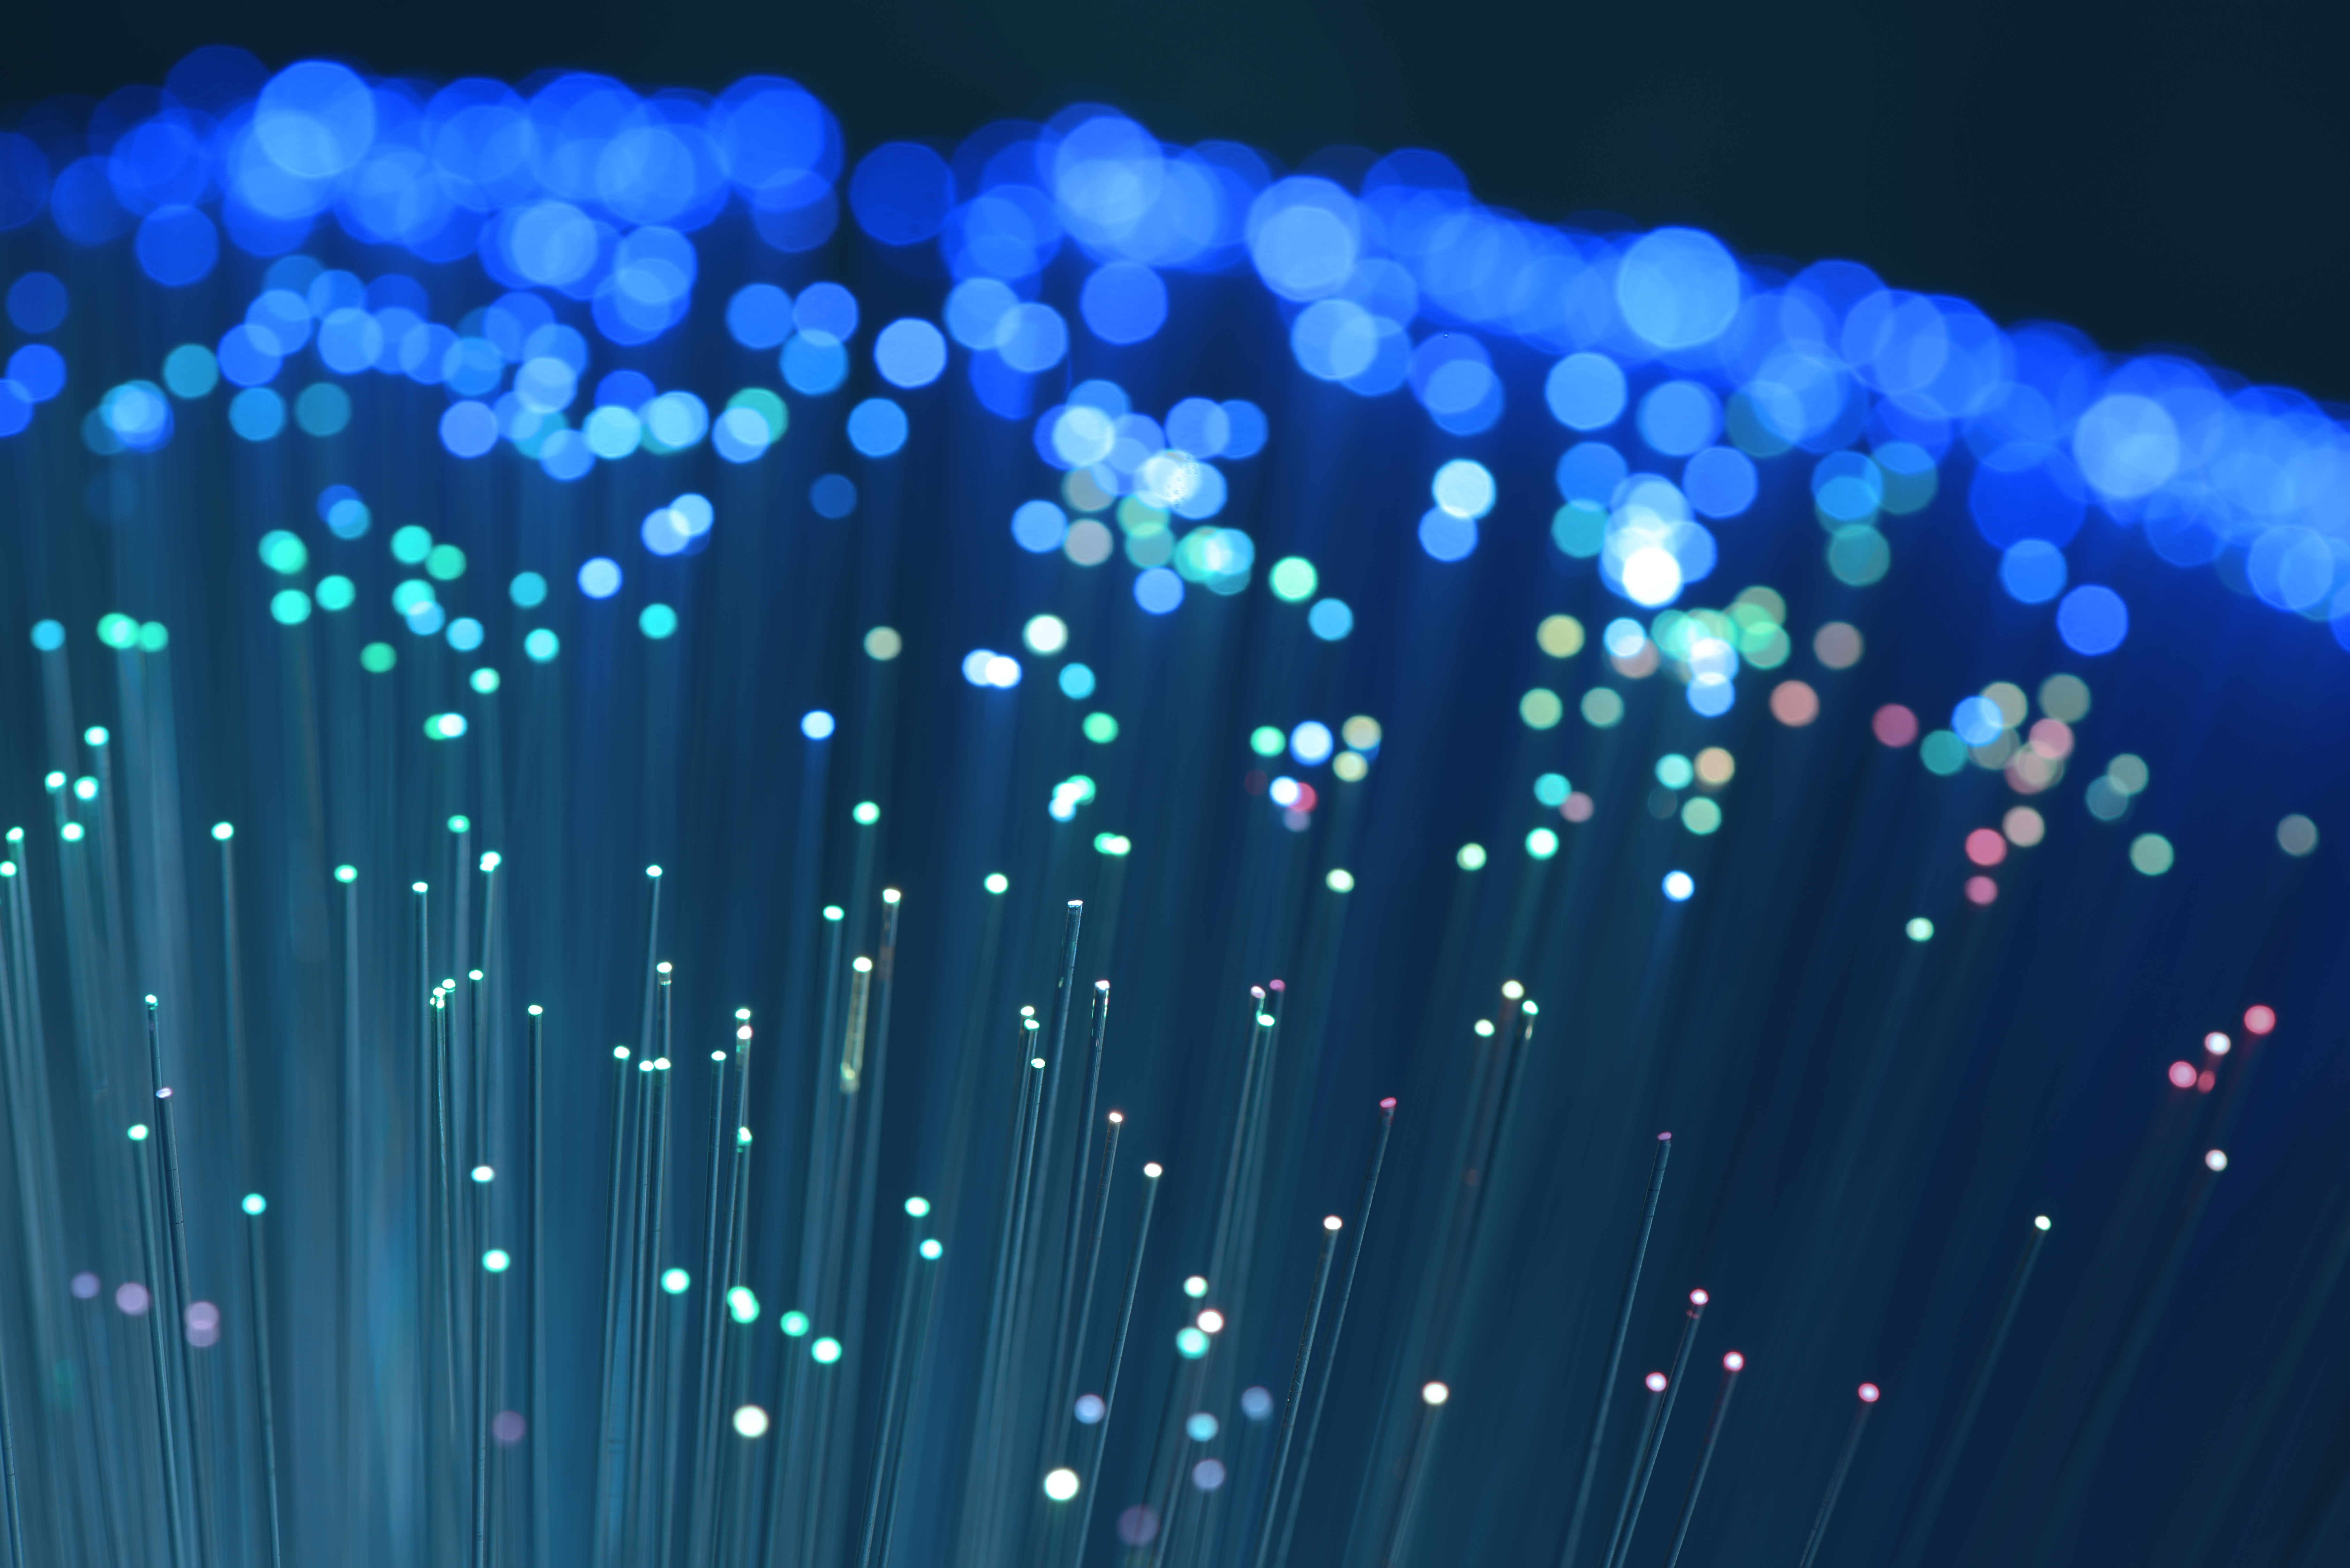
\includegraphics[width=\paperwidth]{wifi7}}
\usebackgroundtemplate{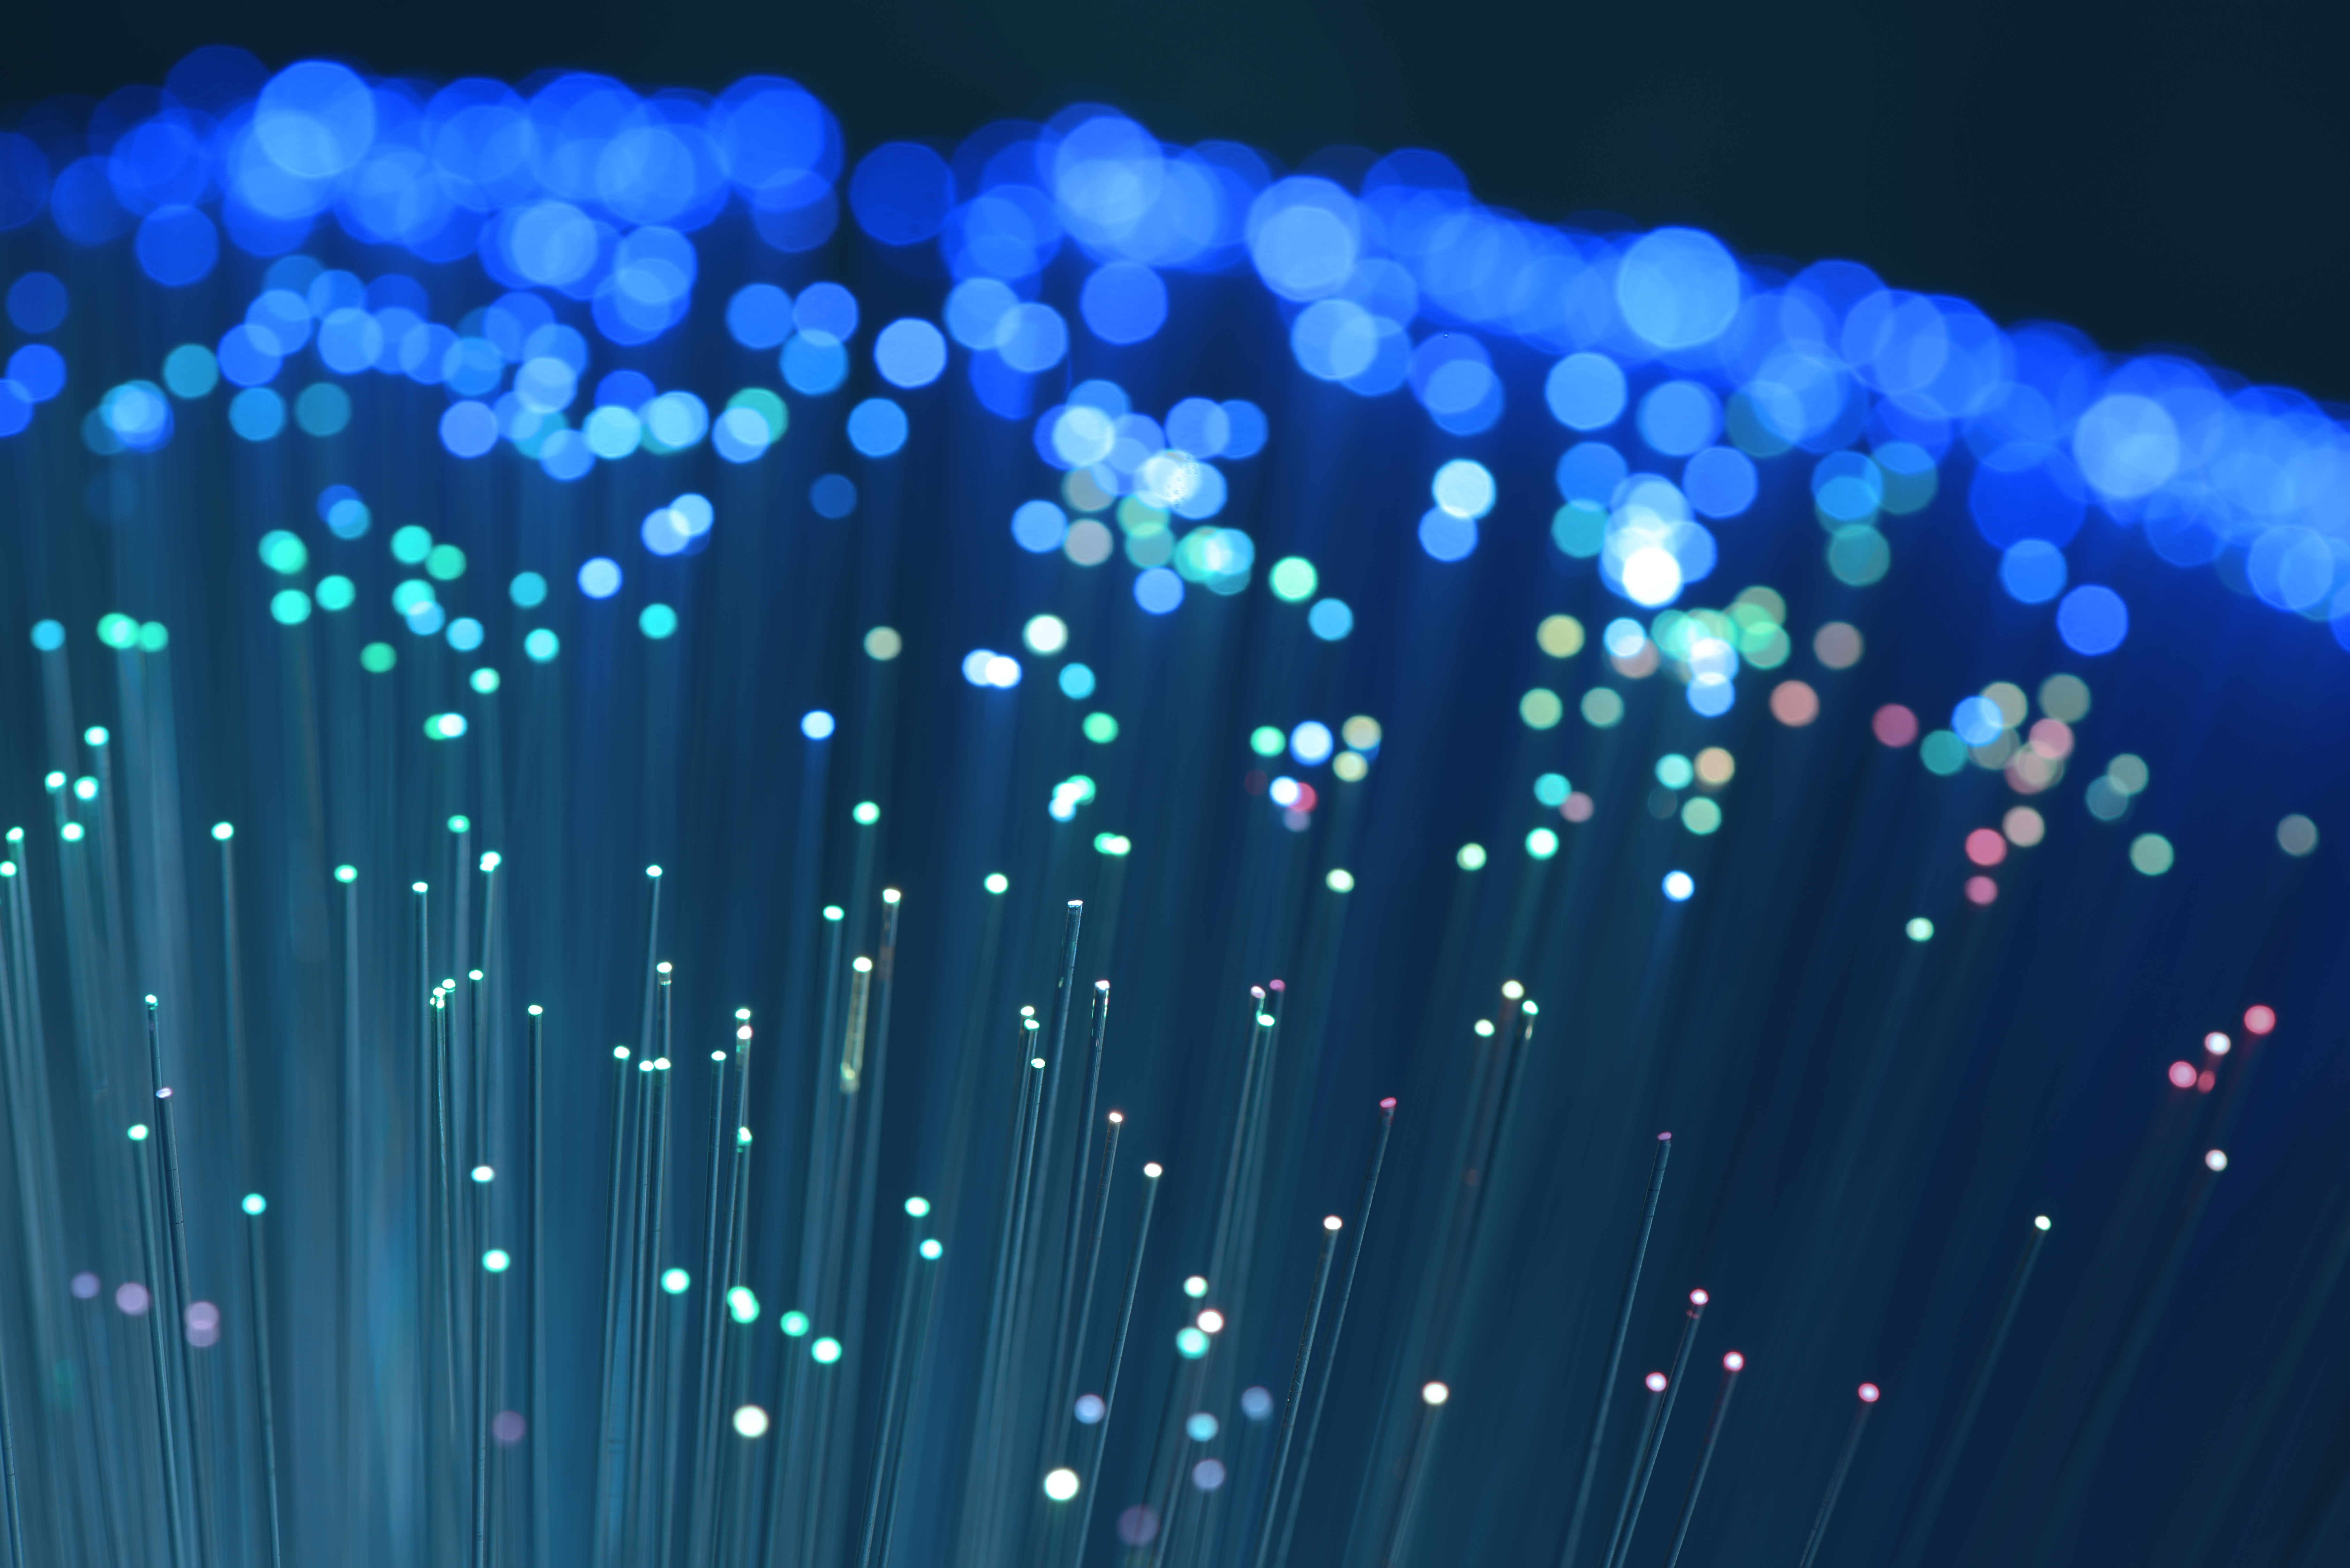
\includegraphics[height=\paperheight]{wifi7}}
\addtobeamertemplate{block end}{}{\vertspace} % White space under blocks
\addtobeamertemplate{block alerted end}{}{\vertspace} % White space under highlighted (alert) blocks
\setlength{\belowcaptionskip}{0ex} % White space under figures
\setlength{\belowdisplayshortskip}{0ex} % White space under equations

\begin{frame}[t] % The whole poster is enclosed in one beamer frame

\begin{columns}[t] % The whole poster consists of three major columns, the second of which is split into two columns twice - the [t] option aligns each column's content to the top

\begin{column}{\sepwid}\end{column} % Empty spacer column

\begin{column}{\firstcolwid} % The first column

%---------------------------------------------------------------
% Introduce the Method
%---------------------------------------------------------------

\begin{alertblock}{The Method of Geometric Optics}
\setbeamercolor{item}{fg=\alertblockitem}
\captionsetup[figure]{labelfont={color=\alertblockcaption}}
\begin{itemize}
\item The idea of the method is to use \textbf{straight lines (rays)} to model waves. 
\\
\begin{centering}
\begin{figure}
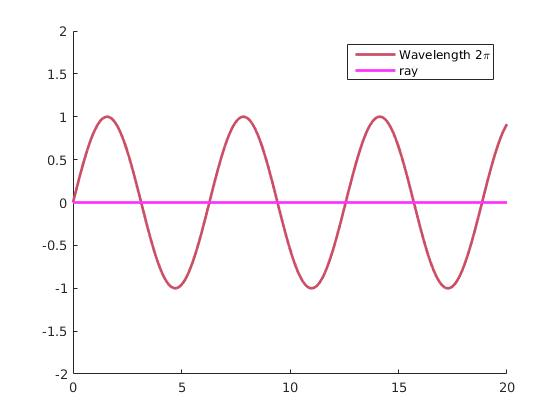
\includegraphics[width=0.85\linewidth]{WaveRay.jpg}
\end{figure} 
\end{centering}
\item \textbf{Rays} are mapped around an environment from source to visualise the path of the waves. An example is given in Figure \ref{fig::rayfield}. 
\\
\begin{figure}
\begin{centering}
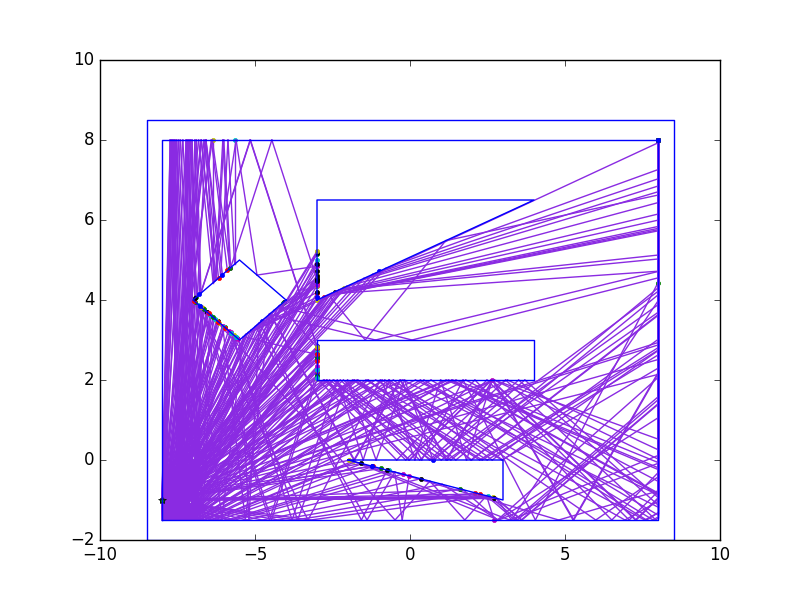
\includegraphics[width=0.85\linewidth]{Rayfield.png}
\caption{\textcolor{black}{Rays propagating from a source and reflecting within an environment. \label{fig::rayfield} }}
\end{centering}
\end{figure}
\item \textbf{Field of rays} is then observed to give an overview of the results in the environment. 
\item Calculations are then made \textbf{along the ray} and hence \textbf{over the ray field} to determine information about the \textbf{properties wave}. 
\item \textbf{Ray-tracing} requires the wave-length to be small relative to the dimensions of the environment.
\end{itemize}
\end{alertblock}
\vertspace


%------------------------------------------------------------------------------
%	Explain the method
%--------------------------------------------------------------------------------

\begin{block}{Why Use the Method?}
\setbeamercolor{item}{fg=\blockitem}
\captionsetup[figure]{labelfont={color=\blockcaption}}
\begin{itemize}
\item An \textbf{advantage} is that the method is \textbf{much faster} to compute than numerical partial differential equation methods for the wave equation, especially for waves with \textbf{small wave lengths}.
\\
\begin{centering}
\begin{figure}[H]
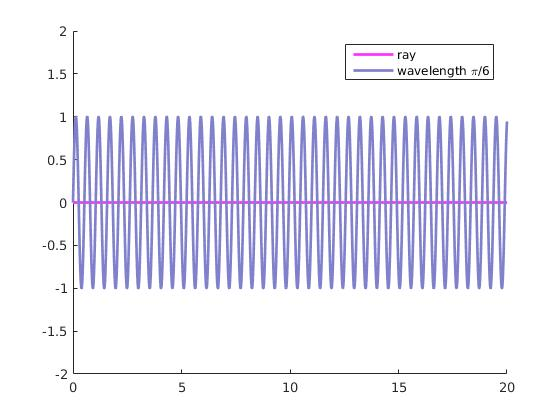
\includegraphics[width=0.45\linewidth]{smallwavelength.jpg} 
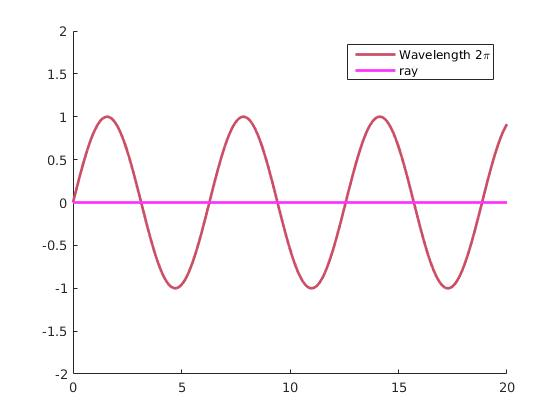
\includegraphics[width=0.45\linewidth]{WaveRay.jpg} 
\caption{\textcolor{\blockcaption}{Using a ray approximation for a wave is better when the wavelength is small.} }
\end{figure}
\end{centering}
\item A \textbf{disadvantage} is that the method requires lots of information about the environment which can be difficult to obtain.
\end{itemize}
\end{block}

%---------------------------------------------------------------

\end{column} % End of the first column

\begin{column}{1.0\sepwid}\end{column} % Empty spacer column

\begin{column}{\twocolwid} % Begin a column which is two columns wide (column 2)

%----------------------------------------------------------------------------------------
%	Introduce The Project
%----------------------------------------------------------------------------------------
    
\begin{block}{High Frequency Wave Propagation}
\setbeamercolor{item}{fg=\blockitem}
\captionsetup[figure]{labelfont={color=\blockcaption}}
\begin{itemize}
\item A time-independent model for wave propagation is the 
\textbf{Helmholtz equation}:
\begin{equation}
\nabla^2 S(x)+{\underbrace{k}_{\substack{\text{Wave} \\ \text{number}}}}^2S(x)=0.
\end{equation}
\item When the wave number $k=\frac{2\pi}{\lambda}$ is large (i.e $\lambda$-wavelength is small) then the wave can be approximated by the \textbf{Eikonal Equation}:
\begin{equation}
{|\nabla S|}^2=n,
\end{equation}
where n is the refractive index.
\item Hence the wave propagation can be described with the use of rays.
\item High frequency waves require a very coarse mesh for numerical \pde approximations. This makes the method of Geometric Optics more appealing.
\item Wavelength relates to frequency by the following, 

\begin{equation}
\text{Wavelength}=\lambda=\frac{v_p}{f}=\frac{\text{phase velocity}}{ \text{frequency}}
\end{equation} 

Hence when the frequency is high, the wavelength is small, and this meets the requirements for using the method of geometric optics.
\end{itemize}
\end{block}
\vertspace
\captionsetup[figure]{labelfont={color=\alertblockcaption}}
 \setbeamercolor{item}{fg=\alertblockitem}
%----------------------------------------------------------------------------------------
\begin{alertblock}{Application}

\begin{itemize}
\item One real world example of high frequency waves are electromagnetic waves, in particular wifi waves. 
\item Developments in wifi-enabled technologies have resulted in an increased demand for wifi propagation models.
\begin{figure}[H]
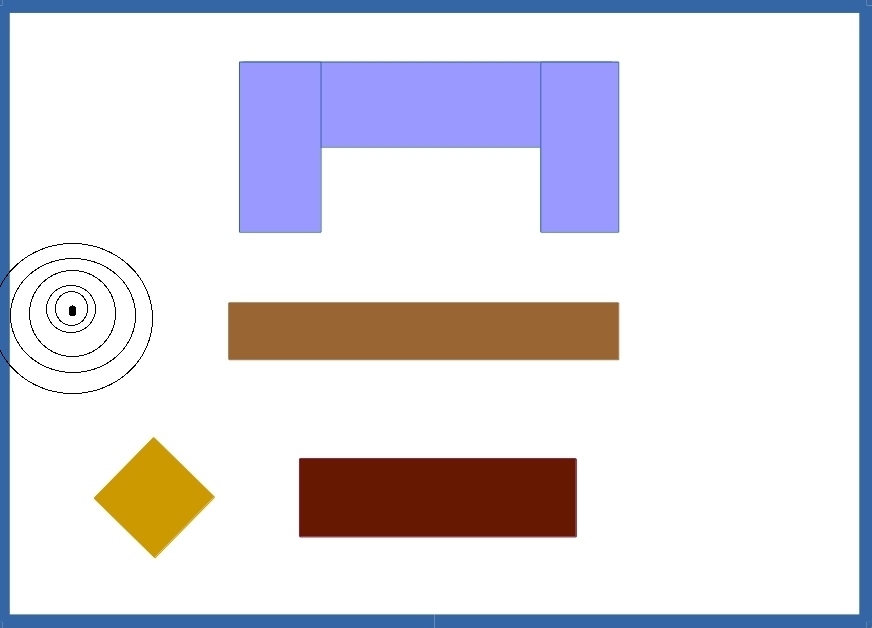
\includegraphics[width=0.7\linewidth]{Room} 
\caption{Template environment in two dimensions. \label{fig::temproom}}
\end{figure}
\item Figure \ref{fig::temproom} gives an example environment with a source radiating wifi waves. 
\item To get an idea of the coverage around the environment the method of geometric optics can be used.
\end{itemize}
\end{alertblock}
%----------------------------------------------------------------
%		MOTIVATION FOR THE RESEARCH
%------------------------------------------------------------
  % Coloured straight line box
% \vspace{-2cm}
% \hspace{0.5in}
% \begin{beamercolorbox}[wd=14in,colsep=0.15cm]{cboxb}
% \end{beamercolorbox}



\end{column}

\begin{column}{\sepwid}
% SPACER COLUMN
\end{column}

\begin{column}{\threecolwid}
\captionsetup[figure]{labelfont={color=\alertblockcaption}}
 \setbeamercolor{item}{fg=\alertblockitem}
\begin{alertblock}{Results }

\begin{figure}[H]
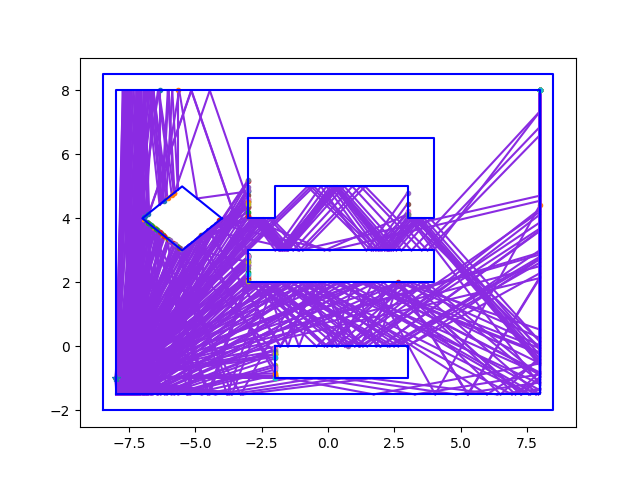
\includegraphics[width=0.4\linewidth]{MultiRay} 
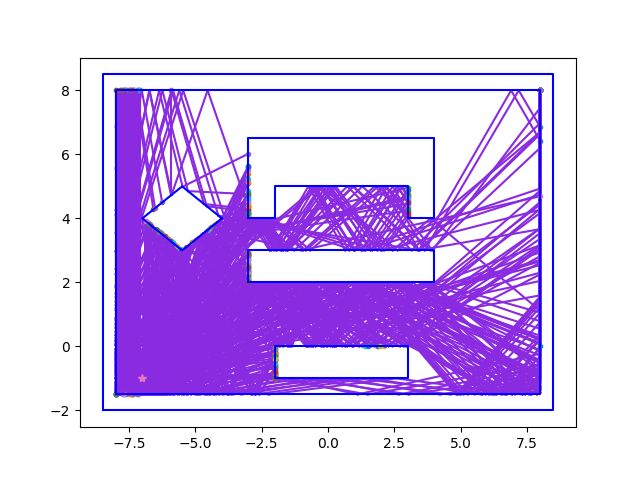
\includegraphics[width=0.4\linewidth]{MultiRay2}
\caption{\textcolor{\alertblockcaption}{The rays propagating from the transmitter and reflecting from two different sources.\label{fig::rayroom}} 
}
\end{figure}

%%%%%%%%%%%%%%EDITEDIT

\begin{itemize}
\item In Figure \ref{fig::rayroom} the method of geometric optics has been applied to Figure \ref{fig::temproom} to visualise the coverage. This has been applied to two different source locations.
\item It is also important to get an idea of the signal strength.
\item This can be calculated along the trajectory of the ray taking into account the attenuation from the distance travelled and from the interactions.
\item Figure \ref{fig::signalcoverage} visualises this signal strength coverage.
\item The signal strength can be calculated along the trajectory of the ray to determine the signal coverage.
\end{itemize}

\begin{figure}[H]
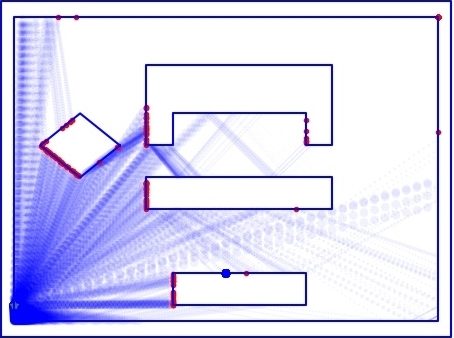
\includegraphics[width=0.4\linewidth]{signalcoverage1}
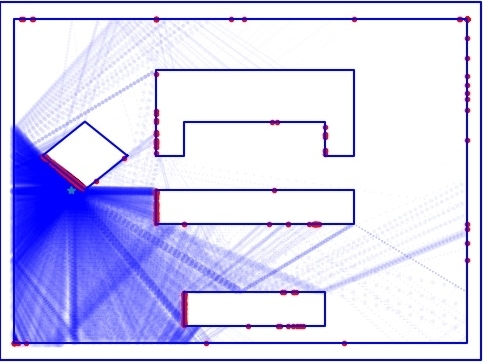
\includegraphics[width=0.4\linewidth]{signalcoverage2} 

\caption{\textcolor{\alertblockcaption}{The signal strength along the ray trajectories. \label{fig::signalcoverage}}
}
\end{figure}
\end{alertblock}

\begin{block}{Future Work}
\captionsetup[figure]{labelfont={color=\blockcaption}}
\setbeamercolor{item}{fg=\blockitem}
\begin{itemize}
\item To improve the estimations further, consider other wave interactions such as diffraction, refraction and scattering. 
\item Refraction often has a high attenuation \cite{aragon2008antennas}, diffraction can be modelled using the geometric theory of diffraction \cite{keller1962geometrical}, and scattering is the most expensive interaction to compute \cite{li2014efficient}.
\item Another future consideration would be to extend the model from the 2 dimensional example to 3 dimensions.
\end{itemize}
\end{block}

%----------------------------------------------------------------------------------------
%----------------------------------------------------------------------------------------
%	REFERENCES
%----------------------------------------------------------------------------------------

\vertspace
\begin{alertblock}{References}
\setbeamercolor{bibliography item}{fg=\alertblockitem}
\nocite{*} % Insert publications even if they are not cited in the poster
\textcolor{\alertblockitem}{
\tiny{\scalebox {.2}{\bibliographystyle{unsrt}}}
%%%%%%EDITEDIT
 \bibliography{posterattempt1.bib}
 % Change the posterattempt1.bib file to change the references. The corresponding \cite{} calls will also need to be changed.
 \vertspace}

\end{alertblock}


%----------------------------------------------------------------------------------------
%	ACKNOWLEDGEMENTS
%----------------------------------------------------------------------------------------

% \begin{block}{Acknowledgements}

% \end{block}

%---------------------------------------------------------------

\end{column} % End of the third column

\end{columns} % End of all the columns in the poster

\end{frame} % End of the enclosing frame

\end{document}
